\csname documentclass\endcsname[../main.tex]{subfiles}
\begin{document}
\chapter{Introduction}
\label{firstcontentpage}
% write more about motivating things before jumping into solution 
% paragraph above to sum up: same as contribution -> can be left out or merged


% open problem
Traditional supervised Machine Learning (ML) models learn to 
predict labels from inputs such as images.
Concept Bottleneck Models (CBMs)~\cite{cbm} and Concept Embedding Models (CEMs)~\cite{cem},
split the original process into predicting a set of human-interpretable
concepts/features present in the input, then predicting the label using these concepts,
which increases the interpretability of the label predictions 
made by a model.
This allows us to 
gain a better understanding of the reasoning behind model  
predictions, 
mitigating some of the downsides associated with using ML models as ``black-box'' models.
This is especially useful in areas where 
decisions made are critical to 
human safety, such as medicine
and criminal justice~\cite{xai-1, xai, xai-2}.

Using concepts aligns the way
CBMs make predictions with the way humans make predictions.
It also makes label mispredictions
human-interpretable, which
can be interpreted as mispredictions in
the concepts. Domain Experts can correct these
mispredicted concepts, rather than having to alter the 
input or model itself to improve predictive accuracy.
During inference time, experts can \textbf{intervene on CBMs} by correcting
the mispredicted concepts, leading to more accurate predicted labels. 
This leads to the problem of determining the concepts to intervene on in order
to achieve the best model performance.

% why it is important and why we should care to solve this (motivation)
Previous studies have shown that the choice of concepts to 
intervene on can have significant impacts on the accuracy of the model~\cite{coop, cbm, ectp}.
Thus it is important to find a good \textbf{policy to determine what concepts we should intervene on}.
Despite this, there has not been much research on developing
methods to find good intervention policies, and 
existing methods do not
take into account the effects of multiple
interventions, where intervening on different combinations
of concepts can have different effects on the accuracy.
Past methods mainly focus on greedy approaches, which
attempt to maximise the effects of each intervention
sequentially.
This includes heuristic-based approaches such as intervening on concepts that minimise the
model's uncertainty~\cite{ coop, ectp}, and IntCEMs use ML to directly learn a greedy policy~\cite{intcem}.
Rather than trying to maximise the effect of each individual 
intervention, we propose that we should 
try to \textbf{maximise the effect of interventions for a given 
budget}, 
which is a limit on the number of interventions.
This
reflects real-life scenarios where
there are limits on how many times we 
can query an expert to intervene on concepts, and 
we want to maximise the predictive 
performance of the CBM after those interventions.


% your research question(s)
Following the successes of \textbf{non-greedy solutions 
using 
Reinforcement Learning} (RL)~\cite{rl} over
greedy solutions in similar 
decision-making problems~\cite{gsmrl, non-greedy-2, non-greedy-1},
we hypothesise that non-greedy policies
yield more optimal solutions as they maximise 
the predictive accuracy after a number of interventions rather than at each step.
Thus we investigate the problem of
finding a non-greedy policy to determine
the set of concepts to intervene on for a budget which
maximises the predictive performance of the CBM.

% The key technical idea (not abstract but technical detail) and innovation that you did that enabled you to answer your question
We utilise RL
to learn a policy that maximises
the model accuracy after a set number of interventions,
using the accuracy of the CBM as a reward to train the RL agent.
In order
to guide the agent throughout the intervention process,
we use a variant of normalising flow models~\cite{normalizing-flows} to model the distribution of concepts. 
This allows us to compute the \textbf{conditional likelihood of concepts}, using it to provide \textbf{intermediate rewards and auxiliary information} to the RL agent.

% How you did it (methodology)
After pre-training a surrogate model to learn the distribution of concepts,
we train a Reinforcement Learning agent in conjunction with a CEM, which we name RLCEM.
RLCEM learns a 
non-greedy intervention policy, using
the expected information gain from the surrogate model
as a reward, and a final reward based on the 
accuracy of the CBM after all interventions.


An overview of the general structure of our RLCEM is in Figure~\ref{fig:rlcem-overview}.
The RL agent learns to output interventions, which are 
used to train the CEM to increase sensitivity of 
CEM to interventions. After all interventions from the RL agent,
the CEM prediction is used to calculate the final
reward to train RL agent. Additionally, a pre-trained surrogate model
is used to calculate intermediate rewards to guide the RL agent to make more optimal intermediate interventions.

\begin{figure}[!ht]
    \centering
    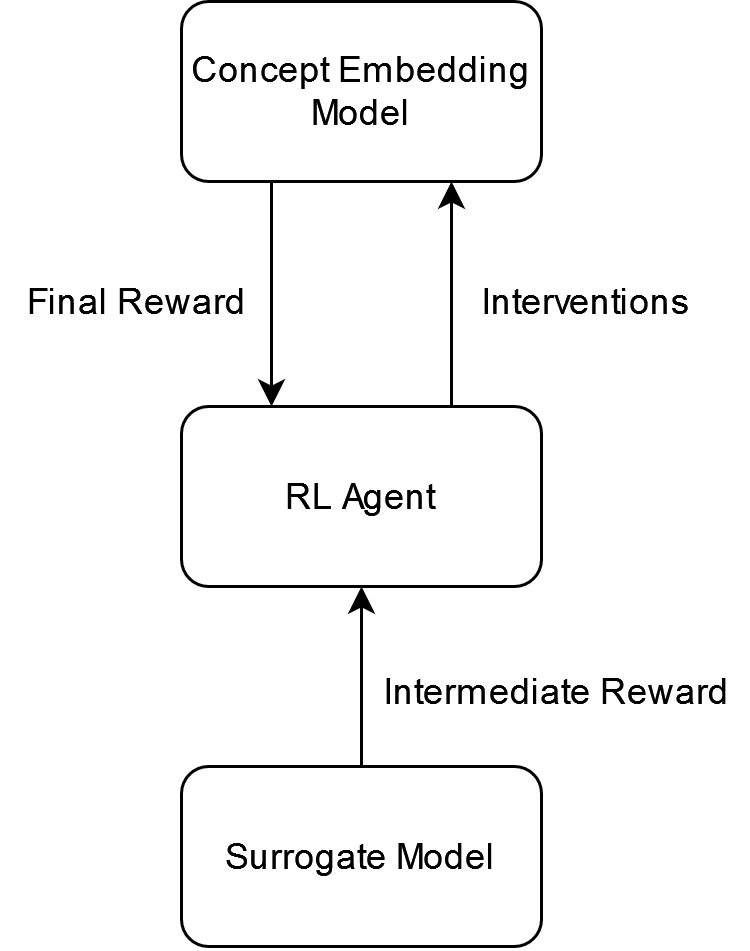
\includegraphics[width=0.4\textwidth]{figs/method/rlcem_overview.png}
    \caption{An overview of the structure of RLCEM. The RL agent samples interventions for the CEM, which is used to calculate
    the final reward to train the agent. The surrogate model is used to calculate intermediate rewards
    to train the agent.}
    \label{fig:rlcem-overview}
\end{figure}

% What the results were
To evaluate this approach, we train RLCEM on two different datasets
and compare its performance to IntCEM and CooP,
the state-of-the-art greedy intervention policies.
We show that this approach can outperform existing greedy policies
for different budgets, achieving better model performance
after a set number of interventions and reaching \textbf{similar or better
predictive accuracy with 25\% less interventions}.



% % What impact could your contributions have
To sum up, this project makes the following contributions:
\begin{itemize}
    \item We introduce budgets into the problem
    of finding intervention policies and show that non-greedy policies can outperform greedy policies.
    \item Show that RLCEMs can
    can learn a non-greedy intervention policy
    with better intervention performance than existing methods. At the same time, the model maintains similar performance under 
the absence of interventions. 
    % \item Standardise the RL environment of RLCEMs inheriting from the Gymnasium Interface~\cite{gymnasium} which
    % can be used in future research in RL-based intervention policies.
\end{itemize}

However, we note that
RLCEM has limitations: it has a 
higher time complexity and its performance is very dependent on the surrogate model, which 
affects the robustness of the method. Nevertheless, it is a viable method that can be used to learn more optimal non-greedy intervention policies than existing policies.

In Chapter~\ref{chapter-2}, we go over existing methods for learning 
intervention policies and why they do not answer our research question. In Chapter~\ref{chapter-3}, we explain our proposed solution: RLCEM to learn a non-greedy intervention policy for different budgets.
In Chapter~\ref{chapter-4}, we evaluate the performance of our RLCEM against existing intervention policies, showing that it outperforms the current methods that learn greedy intervention policies.
Lastly, in Chapter~\ref{chapter-5}, we conclude our work and propose potential future directions.

% \textbf{Terminology}
% The term ``concepts'' hereafter strictly refers to the labelled concepts present
% in the annotated dataset
% that are used to make label predictions
% . For example, in a dataset of identifying birds,
% these concepts include ``has a red beak'', ``has white feathers'', etc.
% Other similar terms such as ``features'', ``attributes'', do not refer to the same thing
% and will not be used interchangeably with
% "concepts''.

% successfully develops a novel approach in using
% Reinforcement Learning to learn a non-greedy intervention policy 
% for different budgets,
% where we successfully show that our RL-based approach
% learns non-greedy policies that can outperform existing
% greedy policies for different budgets, 

%  We model the costs
% associated with interventions and budgets for interventions, which are constraints present in
%  real life
% applications, and set the main research question to be
% determining the concepts to intervene on for different budgets for a CEM
% to maximize its performance.

% To answer the above question, we first investigate the differences between greedy and non-greedy policies,
% proving that non-greedy algorithms can outperform
% their greedy counterparts. We then build a Reinforcement Learning agent
% that learns to select the next concept to intervene in order to maximize the model's performance for a given budget.
% To guide the agent throughout the intervention process, we utilize surrogate models that model
% the conditional distribution of concepts. A detailed description of these models are in Section~\ref{method:rlcem}.
% These surrogate models guide the RL agent throughout the intervention
% process by rewarding the agent for intervening on concepts that lead to higher probabilities of
% intervened concepts, and provide auxiliary information about the unintervened concepts
%  in order for the agent to make more informed decisions.
% % The output of these surrogate models are then used by a Reinforcement Learning agent in order to
% % perform sequential intervention decisions to maximize the final performance, which is trained
% % in conjunction with a CBM in order to increase the sensitivity of the CBM to
% % the interventions. 
% We augment CEMs with this RL agent and a pretrained surrogate model to form RLCEM, 
% and train the CEM and the RL agent simultaneously, which helps learn a non-greedy policy
% and increase the sensitivity of the CEM to these interventions.

% The results show that such RLCEMs
% outperform existing models when intervened using the learnt policy, while achieving 
% similar performance
% under the absence of interventions. This project successfully demonstrates the how a non-greedy 
% policy can be learnt using Reinforcement Learning and surrogate models that 
% outperforms existing greedy policies for different budgets, showing that Reinforcement Learning
% is a viable approach for learning more optimal intervention policies.

\end{document}